\documentclass[ openright,titlepage,numbers=noenddot,headinclude,twoside,%
                footinclude=true,cleardoublepage=empty,abstractoff,%
                BCOR=5mm,paper=a4,fontsize=11pt,%
                ngerman,american,%lockflag%
]{scrreprt}
\usepackage{graphicx}
\usepackage{amsmath}
\usepackage[
backend=biber,
style=alphabetic,
sorting=ynt
]{biblatex}
\addbibresource{biblio.bib}
\usepackage{fancyhdr}
\usepackage{braket}
\usepackage{modiagram}
\usepackage{tabularx}

\graphicspath{ {./Figures/} }

\pagestyle{fancy}
\lhead{jose-david creme}
\rhead{TODO 1}
\lfoot{TODO 1}
\rfoot{TODO 1}
%\def\changemargin#1#2{\list{}{\rightmargin#2\leftmargin#1}\item[]}
%\let\endchangemargin=\endlist
\title{Modeling properties of the double exchange model hamiltonian}

\begin{document}
\maketitle
\thispagestyle{fancy}
\chapter{Introduction}

Introduce the following topics
\begin{itemize}
  \item Colossal magnetic resistance
  \item Anomalous behavior of magnetic susceptibility in linear chain of Nickelates
\end{itemize}

\chapter{Double Exchange Hamiltonian}

The double exchange model is used to describe mixed valent transition
metal based molecules. The phenomenology of ferromagnetic and anti-ferromagnetic
behavior in such molecules is captured by the various parameters of the
double exchange model Hamiltonian (Eq:~\ref{eq:demodel}).

\begin{equation}
  \begin{split}
\hat{H} &= \sum_i 2K \hat{S}_{a_i}\cdot\hat{S}_{b_i} \\
        &+ \sum_{\braket{ij}} 2J_a \hat{S}_{a_i}\cdot\hat{S}_{a_j} \\
        &+ \sum_{\braket{ij}} t\left( \hat{c}^{\dagger}_{a_i}\cdot\hat{c}_{a_j} + \text{h.c.}\right ) \\
        &+ \sum_{i,i+1} V_{NN}\left ( \delta_{n_i,0}\ \delta_{n_{i+1},0} \right ) \\
        &+ \sum_{i,i+2} V_{NNN}\left ( \delta_{n_i,0}\ \delta_{n_{i+2},0} \right )
  \end{split}
\label{eq:demodel}
\end{equation}

The above Hamiltonian describes a model with two valence orbitals on each
atom (site) ideally of differnet symmetry (i.e. orthogonal, e.g. $a,b$). A schematic is shown in
Figure:~\ref{fig:deham}.

\begin{figure}[ht]
  \centering
\begin{modiagram}[names]
 \atom[$1$]{left}{
    1s = { 0; up} ,
    2s = { 1; up} ,
 }

 \atom[$2$]{right}{
    1s = { 0; up} ,
    2s = { 1;   } ,
 }
 \node[right,xshift=4mm] at (1sright) {$b$};
 \node[right,xshift=4mm] at (2sright) {$a$};
 \node[left,xshift=-4mm] at (1sleft) {$b$};
 \node[left,xshift=-4mm] at (2sleft) {$a$};

 \draw[<-,gray,semithick]   (2sright) edge[bend right] node [left] {} (2sleft);
 \draw[<->,gray,semithick] (1sright) edge[bend left] node [left] {} (1sleft);
 \draw[<->,gray,semithick] (1sleft) edge[bend left] node [left] {} (2sleft);

 \node[left,xshift=2.3cm, yshift=-9mm] at (1sleft) {$J$};
 \node[left,xshift= 4mm, yshift=5mm] at (1sleft) {$K$};
 \node[left,xshift=2.3cm, yshift=-0mm] at (2sleft) {$t$};

 \end{modiagram}
  \caption{\label{fig:deham} Orbital diagram representing the mail interactions of the double exchange model with two valence orbitals on each atom.}
\end{figure}

In Eq:~\ref{eq:demodel}, the spins of the electrons are represented by $S_a$,
where the subscript $a$ denotes the orbital on which the electron resides.  The
creation and annahilation operators of electrons are represented by
$\hat{c}^{\dagger}$ and $\hat{C}$ respectively. The parameters in the model
Hamiltonian are defined as follows:

\begin{itemize}

\item $K$ - The local exchange integral. This exchange integral represents
  Hund's rule and is always positive. The local exchange favors parallel
  coupling i.e. a local high spin determinant.

\item $J$ - The kinetic exchange interaction between orbitals of symmetry $a$
  on neighboring sites. This integral is responsible of the anti-parallel coupling.

\item $t$ - The kinetic energy integral or the hopping term. The
  transfer of electrons from one atom to the neighboring atom is represented
  by the hopping term. This also favors parallel coupling when taken along with
  the exchange integral $K$.

\item $V$ - The hole repulsion term. This takes into account the repulsion between
  holes which are on neighboring sites $V_{NN}$ or next-nearest neighboring sites $V_{NNN}$. The hole repulsion indirectly takes into account the repulsion between
  electrons occupying nearby sites.\cite{calzado_proposal_2001}

\end{itemize}

\section{Parameter Space}

All the parameters of the model are important for understanding the collective
properties of the double exchange hamiltonian. Here we give the order of magnitude
of all the parameters used keeping in mind that we target molecules based on
transition metal atoms.
Previous studies using \textit{ab initio} methods in order to extract model
parameters for various transition metal atoms such as Cu, Mn, and Ni have
provided realistic order of magnitudes of the values of the parameters.
In the present analysis, we use the full range of values in order to represent
the full range of transition metal atoms.

\begin{table}[h!]
\centering
\begin{tabular}{||c||}
 \hline
 Parameters  \\ [0.5ex]
 \hline\hline
 \\
    $ 0.01\lvert t \rvert \le J \le 0.15\lvert t \rvert $    \\ [1ex]
    $ 0.01\lvert t \rvert \le J \le 0.15\lvert t \rvert $    \\ [1ex]
    $ 0.4 \le K \le 0.8 $                                    \\ [1ex]
    $ V_{NN} = \frac{\alpha}{2r}\ ;\ 0.5 \le \alpha \le 0.8 $ \\ [1ex]
    $ V_{NNN} = \alpha V_{NN} $                                \\ [1ex]
 \hline
\end{tabular}
\label{tab:params}
\caption{Table with range of parameter values.}
\end{table}

Including the hole repulsion term
significantly changes the low energy physics of the model as shown by previous
work\cite{calzado_proposal_2001}. Here we will study the


\chapter{Methodology}

\section{Exact diagonalization}

\section{Projector}

Introduce SLEPc and PETSc.

\section{Effective Hamiltonian}

\section{Real Space Renormalization Group}

\chapter{Results}

\section{Hole repulsion}

%TODO

\subsection{Weight vs J}
\subsubsection{Variation with Nsites}
\subsubsection{Variation with Repulsion}

\begin{figure}[ht]
    \centering
    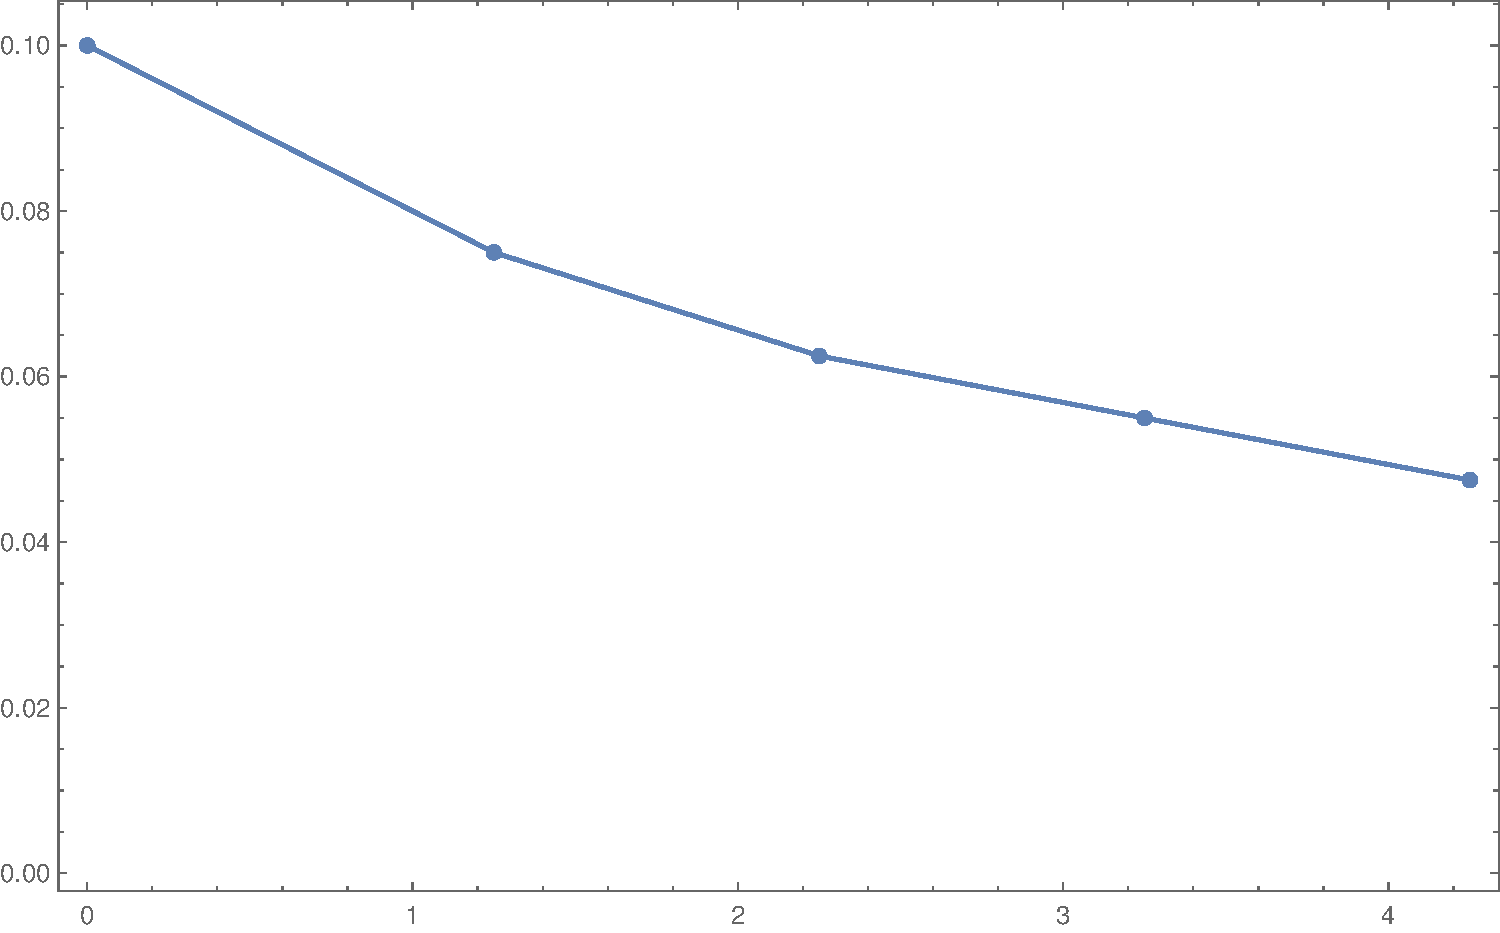
\includegraphics[scale=0.5]{12_4h_J_wmax_vs_xrep.pdf}
    \caption{\label{fig:}Variation of the value of $J$ for which we have a maximum in the weight vs the value of hole repulsion $V$. }
\end{figure}


\begin{figure}[ht]
    \centering
    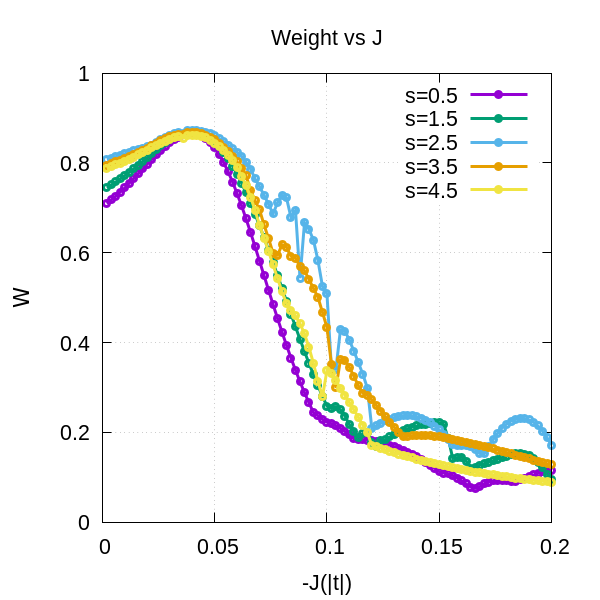
\includegraphics[scale=0.5]{Wmax_vs_J_xrep525.png}
    \caption{\label{fig:}Maximal weight as a function of J for xrep 525. }
\end{figure}

\subsection{$J_{eff}$ vs $J$}
\subsubsection{Variation with Nsites}
\subsubsection{Variation with Repulsion}

\subsection{RSRG}

\chapter{Discussion}

\chapter{Conclusion}

\end{document}



%*************************************************************************
% Bibliographies
%*************************************************************************
\printbibliography
